\documentclass{article}
\usepackage{a4wide}
\usepackage[utf8]{inputenc}
\usepackage{mathtools}
\usepackage{amssymb}
\usepackage[english]{babel}
\usepackage{mdframed}
\usepackage{systeme,}
\usepackage{lipsum}
\usepackage{relsize}
\usepackage{caption}
\usepackage{tikz}
\usepackage{tikz-3dplot}
\usepackage{pgfplots}
\usepackage{harpoon}%
\usepackage{graphicx}
\usepackage{wrapfig}
\usepackage{subcaption}
\usepackage{authblk}
\usepackage{float}
\usepackage{listings}
\usepackage{xcolor}
\usepackage{amsmath}
\usepackage{chngcntr}
\usepackage{amsthm}
\usepackage{comment}
\usepackage{commath}
\usepackage{hyperref}%Might remove, adds link to each reference
\usepackage{url}
\newcommand{\w}{\omega}
\newcommand{\curl}[1]{\mathbf{\nabla}\times \mathbf{#1}}
\newcommand{\grad}{\mathbf{\nabla}}
\newcommand{\dive}[1]{\mathbf{\nabla}\cdot \mathbf{#1}}
%\newcommand{\crr}{\mathfrak{r}}
\usepackage{calligra}

\DeclareMathAlphabet{\mathcalligra}{T1}{calligra}{m}{n}
\DeclareFontShape{T1}{calligra}{m}{n}{<->s*[2.2]callig15}{}
\newcommand{\crr}{\mathcalligra{r}\,}
\newcommand{\boldscriptr}{\pmb{\mathcalligra{r}}\,}
\newcommand{\res}[2]{\text{Res}(#1,#2)}

\title{Handin 8}
\author{Author : Andreas Evensen}
\date{Date: \today}
\definecolor{codegreen}{rgb}{0,0.6,0}
\definecolor{codegray}{rgb}{0.5,0.5,0.5}
\definecolor{codepurple}{rgb}{0.58,0,0.82}
\definecolor{backcolour}{rgb}{0.95,0.95,0.92}

\lstdefinestyle{mystyle}{
    backgroundcolor=\color{backcolour},   
    commentstyle=\color{codegreen},
    keywordstyle=\color{magenta},
    numberstyle=\tiny\color{codegray},
    stringstyle=\color{codepurple},
    basicstyle=\ttfamily\footnotesize,
    breakatwhitespace=false,         
    breaklines=true,                 
    captionpos=b,                    
    keepspaces=true,                 
    numbers=left,                    
    numbersep=5pt,                  
    showspaces=false,                
    showstringspaces=false,
    showtabs=false,                  
    tabsize=2
}

\lstset{style=mystyle}

\begin{document}

\maketitle

\section*{Note:}
In this exercise sheet the Fourier transform, and it's inverse transform is defined below:
\begin{align*}
    \text{Transform: } \tilde{f}(\w) &=\int_{-\infty}^{\infty} f(t)e^{-i\w t}dt\\
    \text{Inverse transform: } {f}(t) &=\frac{1}{2\pi}\int_{-\infty}^{\infty} f(\w)e^{i\w t}d\w
\end{align*}

\section*{Warmup}
\subsection*{a)}
Using Rodrigues formula
\begin{align*}
    L_n(x) = \frac{1}{2^nn!}\frac{d^n}{dx^n}(x^2-1)^n,
\end{align*}and recursion formula:
\begin{align}
    (2l +  1)(1-x^2)^{\frac{1}{2}}P_{l}^m(x) = P_{l - 1}^{m + 1}(x) - P_{l + 1}^{m + 1}(x) \label{eq: recursion}
\end{align}one wish to compute $P_2^1(x)$. Rearranging eq \eqref{eq: recursion} and setting $l =1$ and $m = 0$ gives:
\begin{align*}
    P_{l + 1}^{m + 1}(x) &= -(2l +  1)(1-x^2)^{\frac{1}{2}}P_{l}^m(x) + P_{l - 1}^{m + 1}(x)\\
    P_{2}^1(x) &= -(2 +  1)(1-x^2)^{\frac{1}{2}}P_{1}^0(x) + P_{0}^1(x)\\
    &= -3\sqrt{1- x^2}P_1(x) + (-1)^1\sqrt{1 - x^2}\frac{d}{dx}P_0(x)\\
    &= -3\sqrt{1- x^2}P_1(x) = -3x\sqrt{1 - x^2} 
\end{align*}
\subsection*{b)}
The Heaviside function defined by: $H(x) = \frac{1}{2} +\frac{1}{2}sign(x)$. Computing the Fourier transform is done by the following:
\begin{align*}
    \tilde{H}(\w) &= \int_{-\infty}^\infty dt\left(H(s)e^{-i\w t}\right)\\
    &=\lim_{\epsilon\to 0} \int_{-\epsilon}^\epsilon \frac{1}{2}e^{-i\w t} + \int_{\epsilon}^\infty dt\left( e^{-i\w t}\right)\\
    &=\lim_{\epsilon\to 0} \Bigg[\frac{1}{-2i\w}e^{-i\w t}\Bigg]_{t = -\epsilon}^\epsilon  + \Bigg[\frac{e^{-i\w t}}{-i\w}\Bigg]_{t = \epsilon}^\infty\\
    \tilde{H}(\w) &= p.v\left(\frac{i}{\w}\right) +\pi\delta(\w),
\end{align*}where $p.v(x)$ denotes Cauchy's principal value of $x$. The Laplace transform is thus defined by:
\begin{align*}
    \hat{H}(s) &= \int_0^\infty e^{-sx}H(x)dx\\
    &=\lim_{\epsilon\to0}\left(\underbrace{\frac{1}{2}\int_0^\epsilon e^{-sx}dx}_{ = 0} + \int_{\epsilon}^{\infty} e^{-sx}dx\right)\\
    \hat{H}(s)&= \lim_{\epsilon\to0}\Bigg[\frac{e^{-sx}}{-s}\Bigg]_{x = \epsilon}^{\infty} = \frac{1}{s}.
\end{align*}

\subsection*{c)}
\begin{align*}
    f(t) = \begin{cases}
        1-t; t\in[0,1]\\
        t+1; t\in[-1,0)\\
        0; \text{ otherwise}
    \end{cases}
\end{align*}
\begin{comment}
Computing the Fourier transform:
\begin{align*}
    \tilde{f}(s) &=\int_{-\infty}^{\infty}f(t)e^{-ist2\pi}dt\\
    &= \int_{-1}^0 (t+1)e^{-its2\pi}dt + \int_{0}^1(1-t)e^{-its2\pi}dt\\
    &= \int_{-1}^0 e^{-its2\pi}dt + \int_{-1}^0 te^{-its2\pi}dt + \int_{0}^1e^{-its2\pi}dt - \int_{0}^1te^{-its2\pi}dt\\
    &= \underbrace{\Bigg[\frac{e^{-its2\pi}}{-is2\pi}\Bigg]_{-1}^0  + \Bigg[\frac{e^{-its2\pi}}{-is2\pi}\Bigg]_{0}^1}_{I_1} - \int_{0}^1te^{-its2\pi} dt + \int_{-1}^0te^{-its2\pi}dt\\
    &= I_1 - \Bigg[\frac{te^{-its2\pi}}{-is2\pi}\Bigg]_{t = 0}^{1} + \int_{0}^1\frac{e^{-its2\pi}}{-is2\pi} dt + \Bigg[\frac{te^{-ist2\pi}}{-is2\pi}\Bigg]_{t = -1}^0 - \int_{-1}^0\frac{e^{-its2\pi}}{-is2\pi}dt\\  
    &= I_1 - \frac{e^{-is2\pi}}{-is2\pi} + \int_{0}^1\frac{e^{-its2\pi}}{-is2\pi} dt + \frac{e^{is2\pi}}{-is2\pi} - \int_{-1}^0\frac{e^{-its2\pi}}{-is2\pi}dt\\  
    &= I_1 - \frac{1}{s\pi}\sin(s2\pi) + \int_{0}^1\frac{e^{-its2\pi}}{-is2\pi} dt- \int_{-1}^0\frac{e^{-its2\pi}}{-is2\pi}dt\\
    &= -\frac{-e^{is2\pi} + e^{-is2\pi}}{-2\pi i s} - \frac{1}{s\pi}\sin(s2\pi) + \int_{0}^1\frac{e^{-its2\pi}}{-is2\pi} dt- \int_{-1}^0\frac{e^{-its2\pi}}{-is2\pi}dt\\
    &=  - \frac{2}{s\pi}\sin(s2\pi) + \int_{0}^1\frac{e^{-its2\pi}}{-is2\pi} dt- \int_{-1}^0\frac{e^{-its2\pi}}{-is2\pi}dt\\
    &=  - \frac{2}{s\pi}\sin(s2\pi) + \Bigg[\frac{e^{-its2\pi}}{4s^2\pi^2}\Bigg]_{0}^1- \Bigg[\frac{e^{-its2\pi}}{4s^2\pi^2}\Bigg]_{-1}^0\\
    &=  - \frac{2}{s\pi}\sin(s2\pi) - \frac{1}{4\pi^2s^2}\sin(2\pi s)\\
    &=  -\sin(2\pi s)\left( \frac{2}{s\pi} + \frac{1}{4\pi^2s^2}\right)
\end{align*}
\end{comment}
\begin{align*}
    \tilde{f}(\w) &= \int_{-\infty}^\infty dt\left(f(t)e^{-i\w t}\right)\\
    &= \int_{-1}^0 (t+1)e^{-i\w t}dt + \int_{0}^1(1-t)e^{-i\w t}dt\\
    &= \int_{-1}^0 e^{-i\w t}dt + \int_{-1}^0 te^{-i\w t}dt + \int_{0}^1e^{-i\w t}dt - \int_{0}^1te^{-i\w t}dt\\
    &= \int_{-1}^1 e^{-i\w t}dt + \int_{-1}^0 te^{-i\w t}dt - \int_{0}^1te^{-i\w t}dt\\
    &= \Bigg[\frac{e^{-i\w t}}{-i\w}\Bigg]_{-1}^1 +\Bigg[\frac{te^{i\w t}}{-i\w}\Bigg]_{ -1}^1 - \int_{-1}^0 \frac{e^{-i\w t}}{-i\w}dt - \Bigg[\frac{te^{-i\w t}}{-i\w}\Bigg]_{0}^1 + \int_{0}^1\frac{e^{-i\w t}}{-i\w}dt\\
    &= \Bigg[\frac{e^{-i\w t}}{-i\w}\Bigg]_{-1}^1 +\Bigg[\frac{te^{i\w t}}{-i\w}\Bigg]_{ -1}^1 - \Bigg[\frac{e^{-i\w t}}{-\w^2}\Bigg]_{-1}^0 - \Bigg[\frac{te^{-i\w t}}{-i\w}\Bigg]_{0}^1 + \Bigg[\frac{e^{-i\w t}}{-\w^2}\Bigg]_{0}^1\\
    &= \frac{4}{\w}\sin(\w) + \frac{2}{\w^2}\left(\cos(\w) - 1\right)
\end{align*}
\begin{comment}
\begin{figure}[H]
    \centering
    \begin{tikzpicture}[scale = 0.8]
        \draw[dashed, black!30, step = 0.5] (-5, -2) grid (5, 5);
        \draw[color = red, domain= 0:1] plot(\x, 1 - \x); 
        \draw[color = red, domain= -1:0] plot(\x, 1 + \x); 
        \draw[color = red, domain= -5:-1] plot(\x, 0); 
        \draw[color = red, domain= 1:5] plot(\x, 0) node[right]{$f(t)$}; 
        \draw[color = blue, domain = -5:-0.01] plot(\x, {4 / (\x) * sin(\x r) + 2 /(\x)**2 * (cos(\x r) - 1)});
        \draw[color = blue, domain = 0.01:5] plot(\x, {4 / (\x) * sin(\x r) + 2 /(\x)**2 * (cos(\x r) - 1)}) node[right]{$f(t)$};
    \end{tikzpicture}
    \caption{Plot of $f(t)$ and $\tilde{f}(\w)$}
    \label{fig: task1c)}
\end{figure}
\end{comment}
\begin{figure}[H]
    \centering
    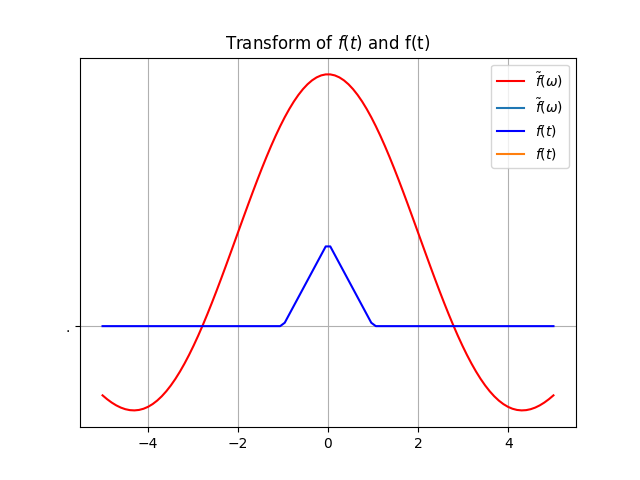
\includegraphics[scale = 0.4]{transform.png}
    \caption{Visualization of $f(t)$ and $\tilde{f}(\w)$}
    \label{fig: task1c}
\end{figure}
\section*{Evaluation of infinite series}
\subsection*{a)}
\begin{align*}
    S = \sum_{n=1}^\infty\frac{1}{n^2}
\end{align*}
Constructing a function $f(z) = \pi\cot(\pi z)\cdot z^{-2}$, one can use the residue theorem to find the sum of the series, and the following contour
\begin{figure}[H]
    \centering
    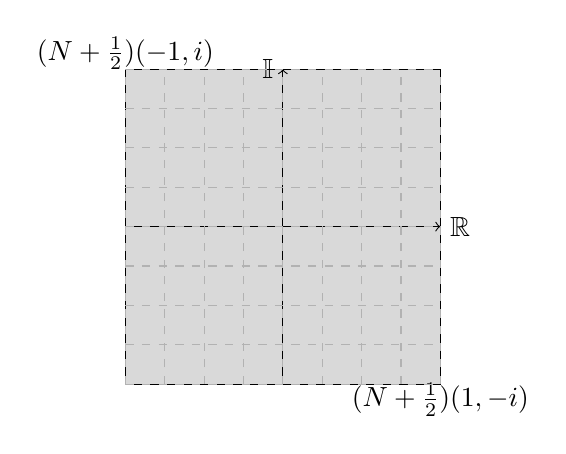
\begin{tikzpicture}
        \draw[fill = gray!30] rectangle (-4,4);
        \node at (-4., 4.2){$(N + \frac{1}{2})(-1, i)$};
        \node at (0, -.2){$(N + \frac{1}{2})(1, -i)$};
        \draw[->] (-4, 2) -- (0,2) node[pos = 1, right] {$\mathbb{R}$};
        \draw[->] (-2, 0) -- (-2,4) node[pos = 1, left] {$\mathbb{I}$};
        \draw[thin, dashed, black!30, step = 0.5] (-4, 0) grid (0,4);
    \end{tikzpicture}
    \caption{Contour used to find the sum of the series.}
    \label{fig: task2a)}
\end{figure}\noindent At $z = 0$ the function, $f(z)$ has a simple pole and one does the Taylor expansion of $cot(z)$ around $z = 0$:
\begin{align*}
    f(z) =\frac{\pi}{z^2}\left(1 -\frac{(\pi z)^2}{2!} + \frac{(\pi z)^4}{4!} - ...\right) = \left(\pi z - \frac{(\pi z)^3}{3!} + ...\right) \cdot\left(... + \frac{a_{-1}}{\pi z} +  a_1(\pi z) + ...\right),
\end{align*}then $a_{-1} = \frac{-\pi^2}{3}$. Using this, one has the following situation:
\begin{align*}
    \frac{\pi^2}{3} &= \sum_{n = -\infty}^\infty\frac{1}{n^2}\\
    &= \sum_{n = -\infty}^1\frac{1}{n^2} + \sum_{n = 1}^\infty \frac{1}{n^2}\\
    &= 2\sum_{n = 1}^\infty \frac{1}{n^2}\\
    \implies\sum_{n = 1}^\infty\frac{1}{n^2} &= \frac{\pi^2}{6}
\end{align*}

\subsection*{b)}
One wish to prove the following identity:
\begin{align*}
    \sum_{n = 0}^\infty \frac{1}{n^2 + a^2} = \frac{\pi}{2a}\coth(\pi a) + \frac{1}{2a^2}\quad ; a > 0.
\end{align*}In order to accomplish this, construct the following function: $f(z) = (z^2 + a^2)^{-1}$ which has simple poles at $z = \pm ai$, and uses the contour defined in \ref{fig: task2a)}:
\begin{align*}
    \sum_{n = -\infty}^\infty f(n) &= - \sum_{z_i} \res{\tilde{f}}{z_i}\\
    &= -\left(\lim_{z\to ai}\frac{(z-ai)\pi\cot(\pi a)}{(z-ai)\cdot(z + ai)} + \lim_{z\to - ai}\frac{(z + ai)\pi\cot(\pi a)}{(z + ai)\cdot(z- ai)}\right)\\
    &= - \left(\frac{\pi\cot(\pi ai)}{2ai} + \frac{\pi\cot(-\pi ai)}{-2ai}\right)\\
    &= \frac{\pi\coth(\pi a)}{a}
\end{align*}
Then one does the following identification:
\begin{align*}
    \frac{\pi\coth(\pi a)}{a} &= \sum_{n = -\infty}^\infty\frac{1}{n^2 + a^2} \\
    &= \sum_{n = -\infty}^{-1}\frac{1}{n^2  + a^2} + \sum_{n = 1}^\infty\frac{1}{n^2 + a^2} + f(0)\\
    &= 2\sum_{n = 1}^\infty\frac{1}{n^2 + a^2} + f(0)\\
    \implies \sum_{n = 1}^\infty\frac{1}{n^2 + a^2} &= \frac{1}{2}\left(\frac{\pi\coth(\pi a)}{a} - f(0)\right)\\
    &= \frac{\pi\coth(\pi a)}{2a} - \frac{1}{2a^2}
\end{align*}

\section*{Laplace transform of the sine cardinal}
\subsection*{a)}
One wish to show the following identity, where $\hat{f}(x)$ is the Laplace transform of $f(t)$:
\begin{align*}
    \int_{s}^\infty dx \left(\hat{f}(x)\right) = \mathcal{L}\left[\frac{f(t)}{t}\right](s)
\end{align*}In order to accomplish this, one suppose the following:
\begin{align*}
    \int_{s}^\infty dx\left( \hat{f}(x)\right) &= \int_{s}^\infty dx\int_{0}^\infty dt\left(e^{-xt}f(t)\right)\\
    \text{Fubinis theorem: } &= \int_{0}^\infty dx \left(f(x)\right) \int_{s}^\infty dt\left(e^{-xt}\right)\\
    &= \int_{0}^\infty dx \left(\frac{f(x)}{x}\right) e^{-sx} = \mathcal{L}\left[\frac{f(t)}{t}\right](s)\\
\end{align*}


\subsection*{b)}
One wish to prove the following transformation:
\begin{align*}
    \mathcal{L}\left[\frac{\sinh(at)}{at}\right](s) = \frac{1}{a}\coth^{-1}\left(\frac{s}{a}\right)
\end{align*}In order to achieve this, one does the following, using the result from a):
\begin{align*}
    g(t) &= \frac{\sinh(at)}{a}\implies \hat{g}(s) = \frac{1}{s^2 - a^2}\\
    \mathcal{L}\left(\frac{\sinh(at)}{at}\right)(s)&=\cdot\mathcal{L}\left(\frac{g(x)}{x}\right)(s)\\
    &=\int_s^\infty \hat{g}(x)dx = \int_s^\infty \frac{1}{x^2 - a^2}dx\\
    &= \int_{\frac{s}{a}}^\infty \frac{a}{a^2u^2 - a^2}du = -\frac{1}{a}\underbrace{\int_{\frac{s}{a}}^\infty \frac{1}{-u^2 + 1}du}_{\coth^{-1}(\frac{s}{a}); \abs{\frac{s}{a}}>1}\\
    &= -\frac{1}{a}\coth^{-1}\left(\frac{s}{a}\right)
\end{align*}
\subsection*{c)}
Noting that $g(t) = \frac{\sin(at)}{a}$, and $\hat{g}(s) = \frac{1}{x^2 + a^2}$, one uses the same trick as before to prove the following identity:
\begin{align*}
    \mathcal{L}\left[\frac{\sin(at)}{at}\right](x) = \frac{1}{a}\cot^{-1}\left(\frac{s}{a}\right).
\end{align*}One does the following set of computations to find the result:
\begin{align*}
    \mathcal{L}\left(\frac{\sin(at)}{at}\right) &= \int_s^\infty \frac{1}{x^2 + a^2}dx\\
    &= \frac{1}{a}\int_{\frac{s}{a}}^\infty \frac{1}{u^2 + 1}du\\
    &=\frac{1}{a}\cot^{-1}\left(\frac{s}{a}\right)
\end{align*}
\end{document}
    